%b  !TEX TS-program = lualatex
% !TEX encoding = UTF-8 Unicode

% This is a simple template for a LaTeX document using the "article" class.
% See "book", "report", "letter" for other types of document.

\documentclass[12pt]{report} % use larger type; default would be 10pt

\usepackage[utf8]{inputenc} % set input encoding (not needed with XeLaTeX)
\usepackage{fontspec}
\setmainfont{Georgia}
\setsansfont{Georgia}
\setmonofont{Georgia}
%\usepackage[none]{hyphenat}
\usepackage{hyphenat}

%%% Examples of Article customizations
% These packages are optional, depending whether you want the features they provide.
% See the LaTeX Companion or other references for full information.

%%% PAGE DIMENSIONS
\usepackage{geometry} % to change the page dimensions
\geometry{a4paper, left=25mm, right=25mm, textwidth=85mm,columnsep=5mm, top=25mm}
\setlength{\parindent}{0pt}
% or letterpaper (US) or a5paper or....
% \geometry{margin=2in} % for example, change the margins to 2 inches all round
% \geometry{landscape} % set up the page for landscape
%   read geometry.pdf for detailed page layout information

\usepackage{subcaption}
\usepackage{graphicx} % support the \includegraphics command and options

\usepackage[parfill]{parskip} % Activate to begin paragraphs with an empty line rather than an indent

%%% PACKAGES
\usepackage{booktabs} % for much better looking tables
\usepackage{array} % for better arrays (eg matrices) in maths
\usepackage{paralist} % very flexible & customisable lists (eg. enumerate/itemize, etc.)
\usepackage{verbatim} % adds environment for commenting out blocks of text & for better verbatim
%\usepackage{subfig} % make it possible to include more than one captioned figure/table in a single float
\usepackage{amsmath}
\usepackage{amsfonts}
% These packages are all incorporated in the memoir class to one degree or another...
\usepackage{lipsum}
%\usepackage{caption}
\usepackage{listings}

%%% HEADERS & FOOTERS
\usepackage{fancyhdr} % This should be set AFTER setting up the page geometry
\pagestyle{fancy} % options: empty , plain , fancy
\renewcommand{\headrulewidth}{0pt} % customise the layout...
\lhead{}\chead{}\rhead{}
\lfoot{}\cfoot{\thepage}\rfoot{}

%%% SECTION TITLE APPEARANCE
%\usepackage{sectsty}
%\allsectionsfont{\sffamily\mdseries\upshape} % (See the fntguide.pdf for font help)
% (This matches ConTeXt defaults)

%%% ToC (table of contents) APPEARANCE
\usepackage[nottoc,notlof,notlot]{tocbibind} % Put the bibliography in the ToC
\usepackage[titles,subfigure]{tocloft} % Alter the style of the Table of Contents
\renewcommand{\cftsecfont}{\rmfamily\mdseries\upshape}
\renewcommand{\cftsecpagefont}{\rmfamily\mdseries\upshape} % No bold!
\usepackage{authblk}

\usepackage{float}

\newcommand{\overbar}[1]{\mkern 1.5mu\overline{\mkern-1.5mu#1\mkern-1.5mu}\mkern 1.5mu}

%%% END Article customizations

%%% The "real" document content comes below...

\title{\textbf{Tunable electronic bands in twisted bilayer NbSe$_2$}}
\author{Conan Birkett}
\affil{Department of Physics, University of Bath, Bath BA2 7AY, United Kingdom}
%\date{} % Activate to display a given date or no date (if empty),
         % otherwise the current date is printed 

\begin{document}
\maketitle
\begin{abstract}
  Following observation of unconventional superconductive effects in twisted bilayer gra\-phene, the novel field of 'twistronics' has seen a rapid progression in theory and experimentation. When a van der Waals heterostructure formed from a bilayer of 2D lattices is twisted at a so-called 'magic-angle', perturbation effects and interlayer tunneling lead to the formation of a flat electronic band at the Fermi level in some materials. These exotic electronic properties mean that these materials have the potential to be exploited as high temperature superconductors or in novel electronic devices. Using a multiorbital tight binding model, we model a bilayer of transition metal dichalcogenide 2H-NbSe$_2$ with interlayer tunneling at various twist angles. We observe splitting of electronic bands at degenerate eigenvalues, leading to flat electronic bands near the Fermi level for some twist angles. Our results show potential for further modelling of twisted bilayer NbSe$_2$ to affirm these promising properties.
\end{abstract}

\newpage

\section*{Introduction}

  In 2018, Cao Y. \textit{et al.,} \cite{Cao2018} realised unconventional superconductivity in bilayer graphene twisted to the 'magic-angle' of 1.1$^\circ$. This catapulted interest and research into graphene and two-dimensional (2D) materials to new heights. The potential of graphene in realising new electronic properties and phases of matter has been extensively explored both theoretically and experimentally \cite{Cao2018, Ghuge2017, Bistritzer2010, Bistritzer2011, Geim2013, Gibney2019, Zou2018}.

  In recent years, focus has been directed at electrical properties of other 2D materials, like transition metal dichalcogenides (TMDCs), and into how combining multiple layers of 2D materials into van der Waals heterostructures can drastically affect their electronic properties \cite{Geim2013}. In particular, a novel field, dubbed 'twistronics' has grown from research into how relative interlayer twist in a van der Waals heterostructure influences the electronic properties of an electronic device \cite{Carr2017}. We examine such a heterostructure constructed from a bilayer of 2-hexagonal niobium diselenide (2H-NbSe$_2$); its monolayer is known to have different electronic properties from a bulk substrate: in particular a metallic electronic band structure, and strong Ising-type spin-orbit coupling (SOC) that locks electron spins into out-of-plane directions \cite{Nakata2016, Xi2016, He2018, Habara2021}.

  We show that perturbations introduced by the modelling of interlayer coupling cause electronic bands to separate and avoid crossing at degenerate values \cite{Verhoeven1996, Cohen-Tannoudji2006}. We examine the effects of the perturbations by taking projections of low energy electronic bands onto unperturbed states (those without interlayer coupling). Further, there are points of interest, particularly at saddle points between the $\Gamma$ and K critical points and near the M critical point, which display flat electronic bands near the Fermi level at relatively large twist angles, much like bilayer graphene. These flat electronic bands are a consequence of the aforementioned perturbation. The high density of states associated with flat electronic bands at the Fermi level is well-studied in the context of novel electronic properties in other materials, in particular magic-angle superconductivity in graphene \cite{Cao2018, Bistritzer2011}.

  Experimentally, it is possible to shift the Fermi level in a 2D system by a few hundred MeV by 'sandwiching' it within a capacitor to introduce an electric field \cite{Díaz-Fernández2017}. Additionally, the large twist angle (compared to magic-angle graphene) at which these effects are observed could be more convenient for experimental realisation, as small twist angles require high precision and result in large Moir\'{e} superlattices \cite{Tao2022}. Our results thus suggest tunable novel electronic properties and potentially flat electronic bands in bilayer NbSe$_2$ that are within experimental reach. However, further work is required in modelling the bilayer, as our model makes use of many non-trivial approximations. Significant improvements to the modelling of interlayer tunneling must be made, and may have a drastic effect on the results presented. With this in consideration, our results are promising and justify further research into twisted bilayer NbSe$_2$.

\section*{Method}
  Our work draws on several published methods on NbSe2 and twistronics. In particular we draw upon the multiorbital tight binding model (TBM) of monolayer NbSe2 from Habara and Wakabayashi \cite{Habara2021}. To model the bilayer with twist and interlayer coupling, we employ the method used in the original magic-angle papers by Bistritzer and MacDonald \cite{Bistritzer2010, Bistritzer2011}, which has been generalised for incommensurate atomic bilayers by Koshino \cite{Koshino2015}. 

\subsection*{Monolayer NbSe2}
  NbSe$_2$ is a two-dimensional (2D) transition metal dichalcogenide (TMDC). Specifically, it belongs to the group V TMDCs with formula $MX_2$ for $M =$ Nb, Ta and $X =$ S, Se \cite{Eui-Hyeok2020}. It has metallic properties with superconductivity in the bulk below critical temperature $T_C \approx 7.2$ K \cite{Xi2016}. It also exhibits a strong spin-orbit coupling (SOC) field, which results in Ising-type SOC, i.e. a strong effective Zeeman field, which holds electron spins in out-of-plane directions \cite{Xi2016}.
%
\begin{figure}[t]
\centering
  \begin{subfigure}[c]{0.475\textwidth}
    \centering
    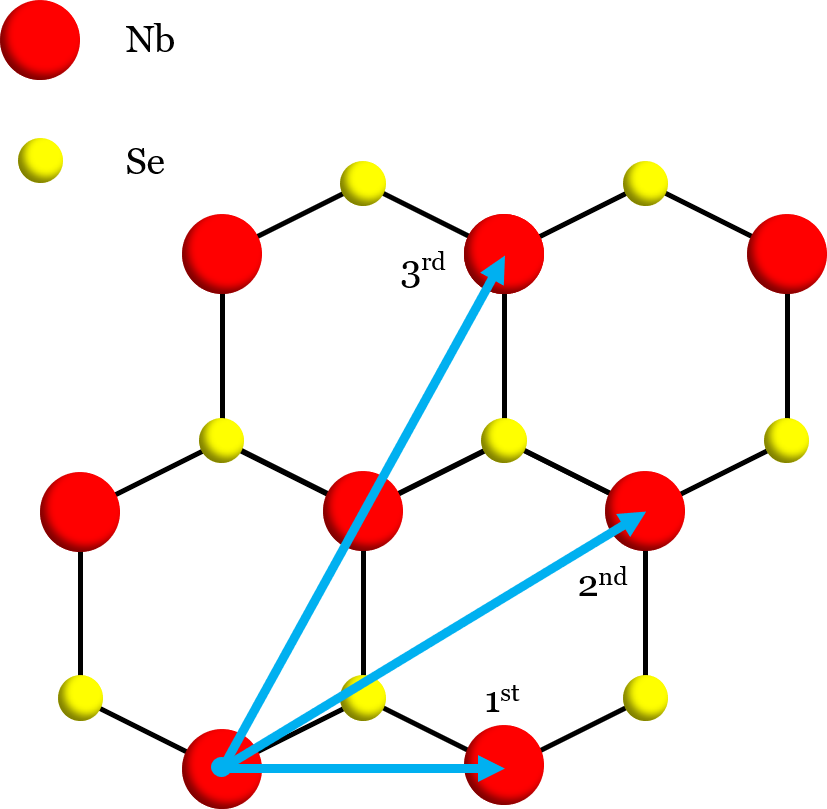
\includegraphics[width=0.95\textwidth]{NbSe_top.png}
    \caption{
    }
  \end{subfigure}
  \hfill
  \begin{subfigure}[c]{0.475\textwidth}
    \centering
    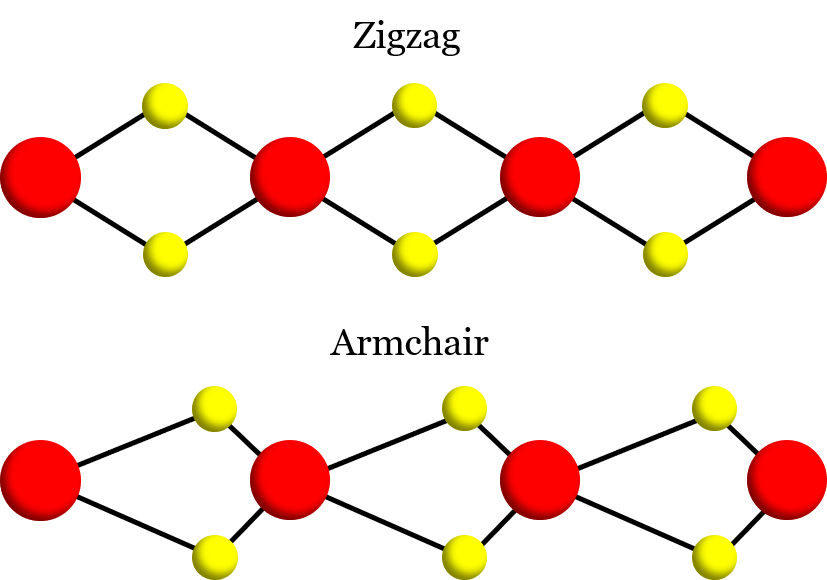
\includegraphics[width=0.95\textwidth]{NbSe_side.png}
    \caption{
    }
  \end{subfigure}
  \caption{
    Monolayer NbSe$_2$: a) Top view of NbSe$_2$ with example nearest neighbours (NN) up to third NN sites. b) Side view of NbSe$_2$ seen from the 'zigzag' and 'armchair' edges (from the bottom and left sides in a) respectively), Se atoms are directly above and below each other in the out-of-plane axis.
  }
\end{figure}

  We employ a TBM of NbSe2, as described by Habara and Wakabayashi \cite{Habara2021}. We take a basis of $d_{z^2}$, $d_{x^2 - y^2}$ and $d_{xy}$ orbitals of the Nb atoms with SOC. These states are dominant in the electronic band near the Fermi level \cite{Conte2019}. As such, this basis is suitable for modelling the behaviour of low-energy electronic states in a NbSe$_2$ monolayer \cite{Habara2021, Conte2019, Liu2013}. An expansion to this basis might include the $p_x$ and $p_y$ orbitals of the Se atoms, This is supported by Liu \textit{et al.,} \cite{Liu2013} who suggest that for group-VIb TMDCs with formula $MX_2$ the $p$ orbitals of the $X$ atoms contribute to the conduction band spin splitting for $M =$ Mo (comparable mass to Nb), but become negligible for heavier transition metals like $M =$ W. Thus introducing the $p$ orbitals of the Se atoms to the TBM could provide some fine tuning to the results, we forgo this addition to aid the simplicity of the model.

  The TBM considers the interactions of these electronic states up to the third nearest neighbour sites. The eigenvalue equation of the TBM is 
  %
      \begin{equation}
        \label{TBM_evalue_eqn}
        \hat{H}(k)\left|u_{n k}\right\rangle=E_{n k}\left|u_{n k}\right\rangle,
      \end{equation}
      %
   where $k=\left(k_{x}, k_{y}\right)$ is the wave-number vector, $E_{nk}$ is the eigenvalue and $n = 1,2,\cdots,6$ is the band index. We define the eigenvector as
   %
      \begin{equation}
          |u_{n k}\rangle=(c_{n k, d_{z^{2}}, \uparrow}, c_{n k, d_{x y}, \uparrow}, c_{n k, d_{x^{2}-y^{2}}, \uparrow}, c_{n k, d_{z^{2}}, \downarrow}, c_{n k, d_{x y}, \downarrow}, c_{n k, d_{x^{2}-y^{2}}, \downarrow})^{T},
      \end{equation}
%
  where $(\cdots)^T$ indicates the transpose of the vector and $c_{nk\tau s}$ is the amplitude at atomic orbital $\tau$ with spin $s$ for the $n$th energy band at wavevector $k$. The monolayer Hamiltonian $\hat{H}(k)$ with spin orbit coupling is then 
  %
      \begin{equation}
        \hat{H}(k)=\hat{\sigma}_{0} \otimes \hat{H}_{\mathrm{TNN}}(k)+\hat{\sigma}_{z} \otimes \frac{1}{2} \lambda_{\mathrm{SOC}} \hat{L}_{z},
        \label{monolayer_hamitonian}
      \end{equation}
%
  with the TBM nearest neighbour Hamiltonian
%
      \begin{equation}
        \hat{H}_{\mathrm{TNN}}(k)=\left(\begin{array}{ccc}
        V_{0} & V_{1} & V_{2} \\
        V_{1}^{*} & V_{11} & V_{12} \\
        V_{2}^{*} & V_{12}^{*} & V_{22}
        \end{array}\right)
      \end{equation}
%
  and spin orbit coupling term
%
      \begin{equation}
        \hat{L}_{z}=\left(\begin{array}{ccc}
        0 & 0 & 0 \\
        0 & 0 & -2 i \\
        0 & 2 i & 0
        \end{array}\right),
      \end{equation}
%
  where $\hat{\sigma}_0$ and $\hat{\sigma}_z$ are Pauli matrices and $\lambda_{\text{SOC}}=0.0784$ eV is the SOC parameter. The potentials $V_0, \cdots, V_{22}$ in the TNN Hamiltonian are functions of $k$ determined from the nearest neighbour hopping vectors with fitting parameters given in the supplementary from Habara \textit{et al.,} \cite{Habara2021}.
  %
\begin{figure}[t]
\centering
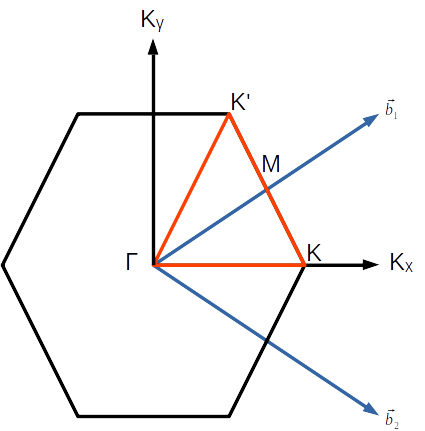
\includegraphics[width=0.6\columnwidth]{1st_BZ.png}
  \caption{
    First Brilloin zone in a hexagonal lattice. shown are: reciprocal lattice vectors $b_1, b_2$, standard critical points $\Gamma, K, K', M$ and wavevector axes $k_x, k_y$. Electronic bands are found for $k$ sampled from the equilateral triangle $\Gamma \rightarrow K \rightarrow M \rightarrow K' \rightarrow \Gamma$ or $\Gamma \rightarrow \Gamma$ shown in red.
  }
  \label{1st_BZ_diagram}
\end{figure}

  The resulting monolayer Hamiltonian $\hat{H}(k)$ is a $6\times6$ block diagonal Hermetian matrix as a function of wavevector $k$. The eigenvalues of this Hamiltonian correspond to the energy of the 6 eigenstates for a given point in reciprocal space $k$. When determining the electronic bands, we take $k$ from slices in the first Brillouin zone along the standard critical points: $\Gamma, K, K', M$. Using Bloch's theorem we can describe the electronic properties of the whole monolayer by considering the region bounded by these points due to the periodicity of potentials in the crystalline lattice and reflectional symmetry. Specifically, we take $k$ on the path formed by the equilateral triangle $\Gamma \rightarrow K \rightarrow M \rightarrow K' \rightarrow \Gamma$ (see FIG \ref{1st_BZ_diagram}), hereafter referred to as $\Gamma \rightarrow \Gamma$. This contains the irreducible Brillouin zone, which is bounded by $\Gamma \rightarrow K \rightarrow M \rightarrow \Gamma$

\subsection*{Modelling a twist}

  Before constructing a twisted bilayer, we first consider a monolayer twisted by some angle $\theta$. A rotation in primitive lattice vectors $a_1, a_2 \rightarrow a_1', a_2'$ corresponds to the same rotation in reciprocal lattice vectors $b_1, b_2 \rightarrow b_1', b_2'$. We can treat this rotation as a rotation of the coordinate system in $k$ space: $(k_x, k_y) \rightarrow (k_x', k_y')$. Then, for some vector $k' \in (k_x', k_y')$, we can describe the same vector $k'$ with respect to our original unrotated wavevector basis $(k_x, k_y)$ by rotating $k'$ inversely to the rotation of the lattice, by $-\theta$.
%
\begin{figure*}[ht!]
\centering
  \begin{subfigure}[t]{0.475\textwidth}
    \centering
    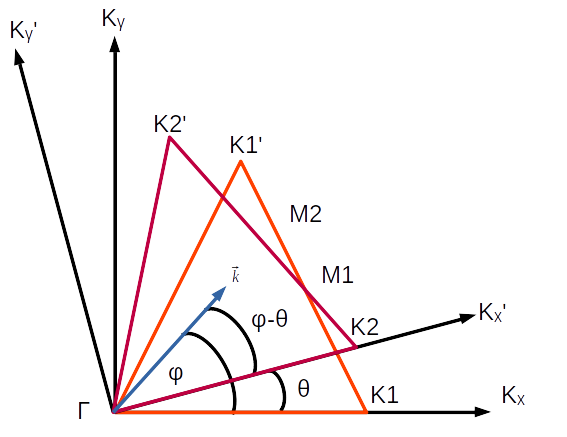
\includegraphics[width=0.95\textwidth]{twisted_triangles.png}
    \caption{
    }
    \label{twisted_triangles}
  \end{subfigure}
  \hfill
  \begin{subfigure}[t]{0.475\textwidth}
    \centering
    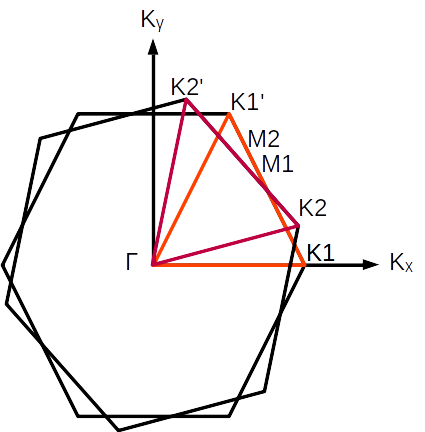
\includegraphics[width=0.95\textwidth]{heterostructure_BZ_path.png}
    \caption{
    }
    \label{heterostructure_BZ_path}
  \end{subfigure}
  \caption{
    Rotated $k$ space paths in Brillouin zone: a) Equilateral triangle from FIG \ref{1st_BZ_diagram} shown in unrotated and relatively rotated (by angle $\theta$) reciprocal coordinate systems. An arbitrary vector $k$ in the rotated basis $(k_x', k_y')$ must first be rotated by $-\theta$ before it can be projected onto the unrotated basis $(k_x, k_y)$. b) First Brillouin zones of both layers at relative angle $\theta$ overlayed. Evaluation of the electronic bands is taken on the set $\Gamma \rightarrow K1 \rightarrow M1 \rightarrow K1' \rightarrow \Gamma \rightarrow K2 \rightarrow M2 \rightarrow K2' \rightarrow \Gamma$ or $\Gamma \rightarrow \Gamma \rightarrow \Gamma$ in $k$ space.
    \label{BZ_triangles}
  }
\end{figure*}

  If we consider the equilateral triangle in reciprocal space $\Gamma \rightarrow K1 \rightarrow M1 \rightarrow K1' \rightarrow \Gamma$ taken on an unrotated basis, we can construct a rotated triangle $\Gamma \rightarrow K2 \rightarrow M2 \rightarrow K2' \rightarrow \Gamma$ as seen in FIG \ref{twisted_triangles}. For the evaluation of electronic bands in a twisted bilayer we sample $k$ from the path $\Gamma \rightarrow K1 \rightarrow M1 \rightarrow K1' \rightarrow \Gamma \rightarrow K2 \rightarrow M2 \rightarrow K2' \rightarrow \Gamma$, or in shorthand $\Gamma \rightarrow \Gamma \rightarrow \Gamma$ (FIG \ref{heterostructure_BZ_path}).

\subsection*{Twisted bilayer}

  NbSe$_2$ monolayers in heterostructures are held together by a weak van der Waals interaction \cite{Geim2013}. This allows for the stacking of multiple layers - specifically a bilayer. Because of the relatively weak bonding between layers it is possible to orient these layers at twist angles relative to each other. Through this rotation, and by interlayer electron tunneling, we aim to explore novel electronic properties in twisted bilayers.

  To describe the electronic states in a twisted bilayer we can initially start with a simple model with no interaction between states in different layers. We construct the Hamiltonian of the whole system by taking a block diagonal Hamiltonian matrix $\hat{H}(k)$ from two monolayer matrices $\hat{H_1}(k)$ and $\hat{H_2}(k')$
%
      \begin{equation}
        \hat{H}(\boldsymbol{k})=\left(\begin{array}{cc}
          \hat{H_1}(\boldsymbol{k}) & 0\\
          0 & \hat{H_2}(\boldsymbol{k'})
        \end{array}\right),
        \label{simple_bilayer_hamiltonian}
      \end{equation}
   %   
  where $\hat{H_2}(k')$ is the Hamiltonian of the second monolayer, which is rotated by angle $\theta$ relative to the first. To find $\hat{H}(k)$ as a function of $k \in (k_x, k_y)$ only, we must rotate the input $k$ to the basis of $k'$ (as described previously) to be evaluated in $\hat{H_2}(k')$. Continuing, we will denote rotated vectors as $v'$ 'prime', where the rotation is relative to its equivalent vector on the 'unrotated layer', $v$. We will also denote these layers by index, layer 1 is unrotated, layer 2 is rotated relative to layer 1.

\subsection*{Interlayer tunneling}
  To model interlayer electron tunneling, we follow the method of Bistritzer and MacDonald \cite{Bistritzer2010, Bistritzer2011} for graphene, which is outlined for a more general case by Koshino \cite{Koshino2015}.

  For reciprocal lattice vectors $b_i, b_i'$, we can show that
  %
  \begin{equation}
    k + G = k' + G',
    \label{inter-layer_k_plus_G}
  \end{equation}
  %
  where $G = m_1 b_1 + m_2 b_2 \text{ and } G' = m_1 b_1' + m_2 b_2',\text{ for } m\in \mathbb{Z}$ are vectors in the reciprocal lattice of the unrotated and rotated layers respectively. This is because a Bloch state on layer one $\phi_k^{(1)}$ is a summation of $e^{i(k+b_i)}$ over reciprocal vectors. Similarily, on layer two $\phi_{k'}^{(2)}$ is a sum over $e^{i(k'+b_i')}$. The system Hamiltonian is described by Fourier components of $G, G'$, so the matrix element $\langle \phi_{k'}^{(2)} | \hat{H} | \phi_{k}^{(1)} \rangle$ is only non-zero if (\ref{inter-layer_k_plus_G}) holds. The derivation of (\ref{inter-layer_k_plus_G}) is as follows:

  First we assume that equivalent unit cells $X$ and $X'$ in both layers have multiple atomic orbitals with real space lattice positions
  %
  \begin{equation}
    \begin{gathered}
    R_X = n_1 a_1 + n_2 a_2 + \tau_X,\\
    R_{X'} = n_1 a_1' + n_2 a_2' + \tau_{X'},
    \end{gathered}
    \label{inter-layer_real_sublattice_positions}
  \end{equation}
%
  for $n_1, n_2 \in \mathbb{Z}$ and primitive lattice vectors $a_1, a_2$ and $a_1', a_2'$ in either layer respectively. $\tau_X$ are the sublattice positions of the atomic states in unit cell $X$.

  We define $| R_X \rangle \equiv \phi(r - R_X)$ as the atomic state of sublattice $X$ localised at real position $R_X$. The interlayer Hamiltonian elements are then
  \begin{equation}
    U = -\sum_{X, X'} T_{X'X}(R_{X'} - R_X) |R_{X'}\rangle \langle R_X|,
    \label{inter-layer_hamiltonian_elements}
  \end{equation}
%
  where the interlayer transfer potential $-T_{X'X}(R_{X'} - R_X)$ is a function of the real space positions of the atomic orbitals, the specifics of this function we shall discuss later.

  We define the Bloch basis in each layer as the summation over unit cells (and thus primitive lattice vectors)
  %
  \begin{equation}
    | k,j,l \rangle = \frac{1}{\sqrt{N_l}}\sum_{R_X}e^{ik\cdot(R_X+\tau_i)}\phi_j(r-R_X-\tau_j, z-z_l),
    \label{inter-layer_real_bloch_basis}
  \end{equation}
%
  for wavevector $k$, sublattice atomic position $j$, layer index $l$ and the number of unit cells in that layer $N_l$. $\phi_j (r - R_X - \tau_j, z-z_l)$ is the wavefunction in the bilayer plane (2D real space) and out of plane (real) directions.

  Our inter-layer hopping Hamiltonian elements are then given by
  %
  \begin{equation}
  \begin{aligned}
    &\langle k',j',l' | U | k, j, l \rangle\\
    &= \frac{1}{\sqrt{N_l N_{l'}}} \sum_{R_X, R_{X'}} e^{ik \cdot (R_X+\tau_j)} e^{-ik' \cdot (R_{X'} + \tau_{j'})} \times \langle \phi_{j'}(r - R_{X'} - \tau_{j'}, z - z_{l'}) | U | \phi_j (r - R_X - \tau_j, z - z_l) \rangle\\
    &=\frac{1}{\sqrt{N_l N_{l'}}} \sum_{R_X, R_{X'}} e^{ik \cdot (R_X+\tau_j)} e^{-ik' \cdot (R_{X'} + \tau_{j'})} \times T(R_{X'}-R_X +\tau_{j'} - \tau_j, z_l' - z_l),
    \label{}
  \end{aligned}
  \end{equation}
%
  where we invoke a two centre approximation for the tunneling potential, the hopping between sites is a function of their real space distance only. We also assume that the the hopping potential $T(\vec{r_{2D}}, z)$ does not depend on the direction of $\vec{r_{2D}}$ i.e. $T(\vec{r_{2D}}, z) = T(|\vec{r_{2D}}|, z)$.

  For a large Moir\'e superlattice period (corresponding to small twist angles), the relative inter-atomic positions for every pair of atomic sites are required, which makes computation far more complex. It is easier to reconstruct the Hamiltonian in reciprocal space. By taking a Fourier transform and sum over $G, G'$ (see appendix) we can show that
  %
  \begin{equation}
    \langle k',j',l' | U | k, j, l \rangle = \sum_{G, G'} t(k'+G', z) \delta_{k-G, k'+G'},
    \label{inter-layer_hopping_elements}
  \end{equation}
  %
  which yields the result in (\ref{inter-layer_k_plus_G}). Note that we also take the Fourier transform of the tunneling potential $T \rightarrow t$ from 2D real space to 2D reciprocal $k$ space. 
  
\subsection*{Tunneling potential and Hamiltonian}

The interlayer tunneling potential $t(k + G, z)$ must model the interaction between states on two atoms on two layers, so we would expect the interlayer hopping to decay in real space. The full modelling of this interaction is involved and beyind the scope of this report. Instead, we can approximately model the tunneling potential $t(k + G, z)$ as a Gaussian in the plane axes in real space and assume the interlayer distance $z$ is constant. This captures the important property of the potential decay in real space, and the Fourier transform of a Gaussian is also Gaussian, which is convenient for conversion to reciprocal space. Our fourier transformed Gaussian is
%
\begin{equation}
  t(k + G) = \frac{C\pi}{A_{UC} r_0^2}e^{- r_0^2 (k + G)/4},
  \label{tunneling_potential_gaussian}
\end{equation}
%
where $A_{UC}$ is the area of the unit cell, $C$ and $r_0$ are fitting constants.

Due to time limitations, we were unable to find suitable fitting parameters for the implementation of this function. So, in our actual numerical results we further approximate the interlayer tunneling potential as a step function with a constant potential of 0.1 eV, which is approximately the order of magnitude expected in TMDC bilayers\cite{Conte2019}. The further approximated potential is
%
\begin{equation}
  t(k + G) =
  \left\{ 
  \begin{array}{lr}
    0.1 \text{ eV}, & \text{if } G \leq b\\
    0 \text{ eV}, & \text{if } G > b
  \end{array} 
  \right\},
  \label{tunneling_potential}
\end{equation}
where $b$ is the reciprocal lattice constant.

As we are taking the interlayer tunneling to be a Gaussian function of $k+G$, we only consider $G, G'$ of magnitude $\leq$ the reciprocal lattice constant $b$, assuming that for $G, G'$ > $b$ the tunneling decays to a negligible value, giving us the step function in (\ref{tunneling_potential}).

The result of this heavy approximation is that for a given $k, k'$ we have seven pairs of permissible $G, G'$ that obey (\ref{inter-layer_k_plus_G}) restricted by (\ref{tunneling_potential}). We define them as follows: $G_0$ is the zero vector; $G_1, G_2$ are equal to reciprocal lattice vectors $b_1, b_2$; $G_{3,\cdots,6}$ continue from reciprocal lattice vectors in a clockwise fashion in 60$^\circ$ intervals. For convenience, we define
%
  \begin{equation}
    G_i^M = G_i - G_i'
    \label{inter-layer_G_M_def}
  \end{equation}
  such that (\ref{inter-layer_k_plus_G}) becomes
  \begin{equation}
    k' = k + G^M
    \label{inter-layer_k_plus_G_M}
  \end{equation}
%
\begin{figure}[t!]
\centering
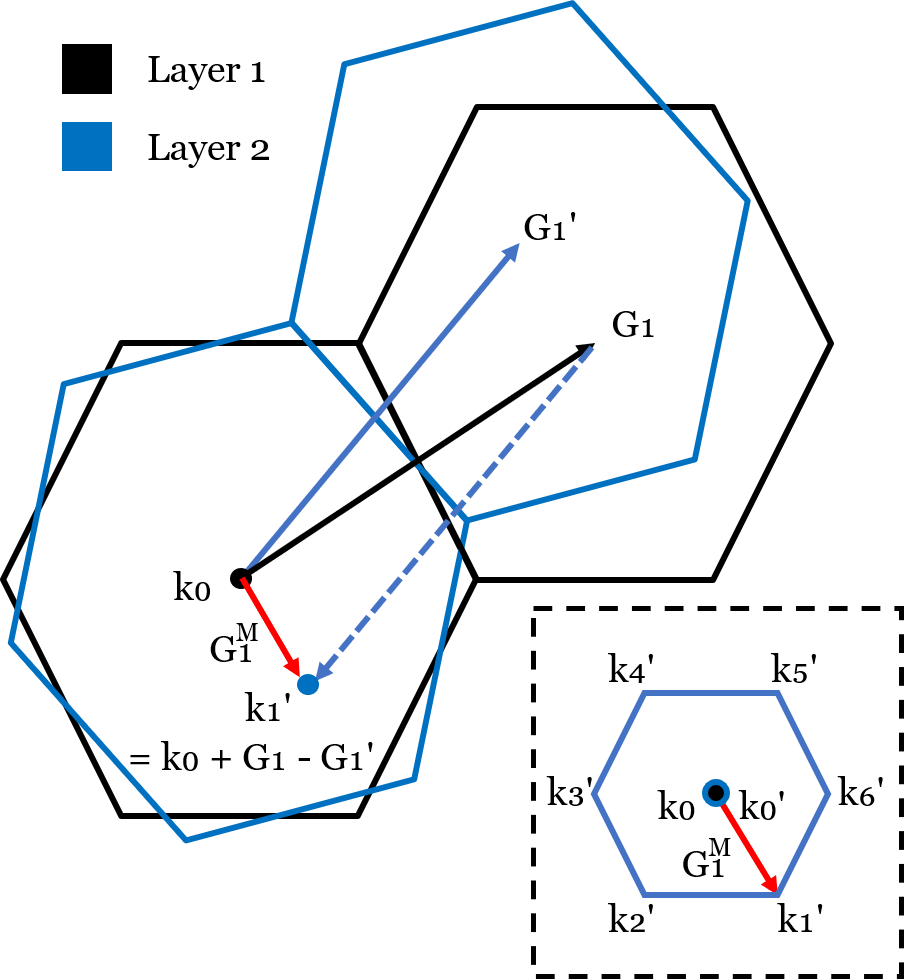
\includegraphics[width=0.6\columnwidth]{k_prime_diagram.png}
  \caption{
    The interlayer tunneling relationship described by (\ref{inter-layer_k_plus_G_M}) implies that for a point $k$ on one layer, there are seven points $k'$ on the other layer between which tunneling is allowed (shown in the insert box)}
  \label{inter-layer_k_prime_diagram}
\end{figure}

  So for a given point $k_0$ on one layer, we have a well defined set of permissible $k'$ points on the other layer between which tunneling is allowed. This is shown in FIG \ref{inter-layer_k_prime_diagram}. We also allow interlayer tunneling between adjacent $k'$ points using the same criteria of (\ref{inter-layer_k_plus_G_M}). This means that (between layers): $k_1$ can tunnel to $k'_0, k'_6 \text{ and } k'_2$; $k_2$ can tunnel to $k'_0, k'_1 \text{ and } k'_3$; \textit{etc}. In only taking the first order of $k'$ points we assume that the tunneling from $k_0$ to further $k'$ points, and tunneling between the further points for which $|G| > b$ is both small and less relevent when evaluating at $k_0$. An improvement to the model could allow a second ring of allowed $k'$ points where the step function (\ref{tunneling_potential}) allows an alternate potential for $b < |G| \leq 2b$.

  Previously our Hamiltonian was a $12\times12$ function of $k$. Now, with the  addition of interlayer tunneling between $k$ on one layer and the 7 allowed $k'$ on the other, we have expanded $k$ into 14 quantum numbers corresponding to these points on both layers. The result is an $84\times84$ block diagonal Hamiltonian with interlayer tunneling perturbations on the off-diagonal blocks between allowed $k, k'$ points. We further assume that the interlayer tunneling is negligible between the $d_xy$ and $d_{x^2-y^2}$ orbitals as they project primarily in the plane axis, so when constructing the Hamiltonian we restrict tunneling to between the $d_{z^2}$ orbitals only.

\subsection*{Avoided crossing in degenerate electronic bands}

\begin{figure}[t!]
\centering
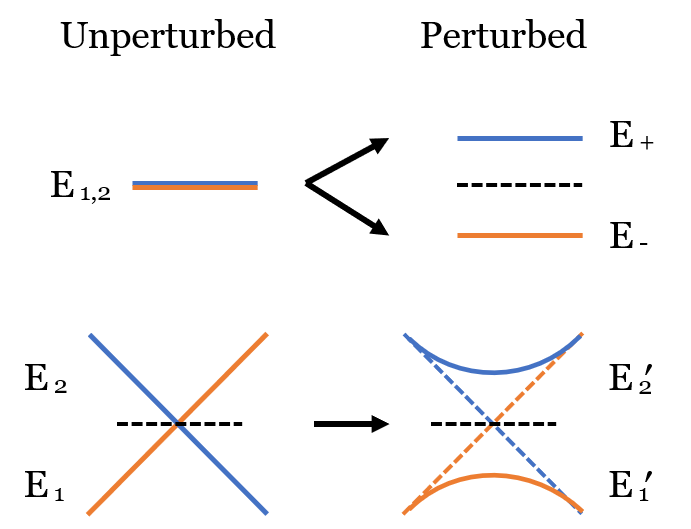
\includegraphics[width=0.6\columnwidth]{splitting_bands_diagram.png}
  \caption{Introducing a coupling perturbation to a Hamiltonian with degenerate eigenvalues results in the eigenvalues separating. In electronic bands this manifests as the bands splitting into two hyperbola at points where they previously would have crossed (degeneracy).}
  \label{splitting_bands}
\end{figure}
%
A well studied phenomena in perturbation theory of quantum mechanics is the splitting of degenerate electronic states under a coupling perturbation \cite{Verhoeven1996, Cohen-Tannoudji2006}. This can be simply explained using an example two state model with Hamiltonian
%
\begin{equation}
  H = \begin{pmatrix}
        E_1 & 0 \\
        0 & E_2 \\
      \end{pmatrix}
      \text{, with eigenvectors }
      \begin{pmatrix}
        1\\
        0\\
      \end{pmatrix},
      \begin{pmatrix}
        0\\
        1\\
      \end{pmatrix},
\end{equation}
%
for some potentials $E_1$, $E_2$. If $E = E_1 = E_2$ then there is twofold degeneracy in the Hamiltonian.

Introducing a simple perturbation in the form of a potential coupling $W$ between the basis states we obtain the modified Hamiltonian
%
\begin{equation}
  H' = H + P =\begin{pmatrix}
    E_1 & 0 \\
    0 & E_2 \\
  \end{pmatrix}
  +\begin{pmatrix}
    0 & W \\
    W* & 0 \\
  \end{pmatrix}
  =\begin{pmatrix}
    E_1 & W \\
    W* & E_2 \\
  \end{pmatrix},
  \label{perturbation_matrix}
\end{equation}
%
upon diagonalising the modified Hamiltonian we find new eigenvalues
%
\begin{equation}
\begin{gathered}
  E_{+, -} = {\frac{1}{2}(E_1 + E_2)} \pm {\frac{1}{2}\sqrt{(E_1-E_2)^2+4|W|^2}},\\
  \text{or, when } E = E_1 = E_2, \quad E_{+,-} = E \pm |W|.
\end{gathered}
  \label{perturbation_energy}
\end{equation}

The perturbation also alters the eigenvectors / eigenstates of the Hamiltonian, they exist as a linear combination of the original unperturbed eigenstates. This principle can be seen in the splitting of electronic (Bloch) bands with the introduction of a perturbation in the form of coupling between basis states. In FIG \ref{splitting_bands} we show an example crossing point (degeneracy) of electronic bands and their modification due to perturbation; the result is that the crossing point becomes two hyperbola and the bands are no longer degenerate \cite{Cohen-Tannoudji2006, Verhoeven1996}. The strength of the band separation is dependent on the difference between two similar energy levels $E_1 - E_2$, that is, the splitting effect is most prevalent at degenerate and nearly degenerate eigenvalues - i.e. near crossing points of electronic bands. As the energy difference between bands increases, the hyperbola asymtotically approach the equivalent unperturbed bands at nondegenerate eigenvalues further from the crossing point.

\subsection*{Implementation}
The numerical implementation of these methods and graphing of their results was performed in Python using the NumPy and Matplotlib libraries. Please see the appendix for further details.

\section*{Results}

\subsection*{Monolayer electronic bands}
%
\begin{figure}[t!]
\centering
  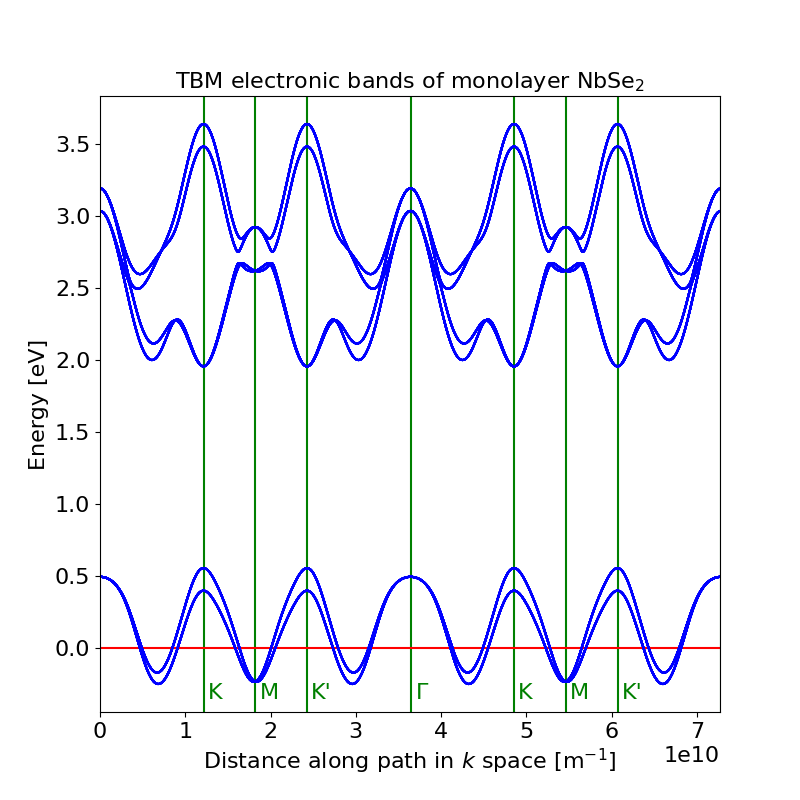
\includegraphics[width=0.6\columnwidth]{monolayer_bands.png}
  \caption{
    Reconstruction of FIG 1 d) from Habara \textit{et al.,} \cite{Habara2021}. 6 Electronic bands are produced from the third nearest neighbour TBM that incorporates $d_{z^2}$, $d_{x^2 - y^2}$ and $d_{xy}$ orbitals of Nb atoms with SOC. The conduction band on the Fermi level (shown in red) tells us that monolayer NbSe$_2$ is metallic. The relatively high SOC in NbSe$_2$ produces the large (meV scale) splitting of bands seen near the $K$ critical points.
  }
  \label{monolayer_bands}
\end{figure}

Initially, we seek to reproduce the tight binding bands from Habara \textit{et al.,} \cite{Habara2021}. Using the matrix elements they provide, we reproduce the six electronic bands from the $d_{z^2}$, $d_{x^2 - y^2}$ and $d_{xy}$ orbitals of the Nb atoms with SOC. The result in FIG \ref{monolayer_bands} is a reproduction of the bands shown in FIG 1 d) of Habara \cite{Habara2021}. Whilst not a novel result, it is a useful benchmark for checking the validity of further results and the implementation of the TBM. Note that Habara \textit{et al.,} sample the bands on a different path in $k$ space, in particular they sample on the path  $M \rightarrow K' \rightarrow \Gamma \rightarrow K \rightarrow M$. So whilst we show the same bands, the $k$ space axis is arranged differently. The NbSe$_2$ monolayer bands predict the electrical properties of the monolayer, in particular that it is metallic.

\subsection*{Bilayer electronic bands}
%
\begin{figure*}[t!]
\centering
  \begin{subfigure}[b]{0.475\textwidth}
    \centering
    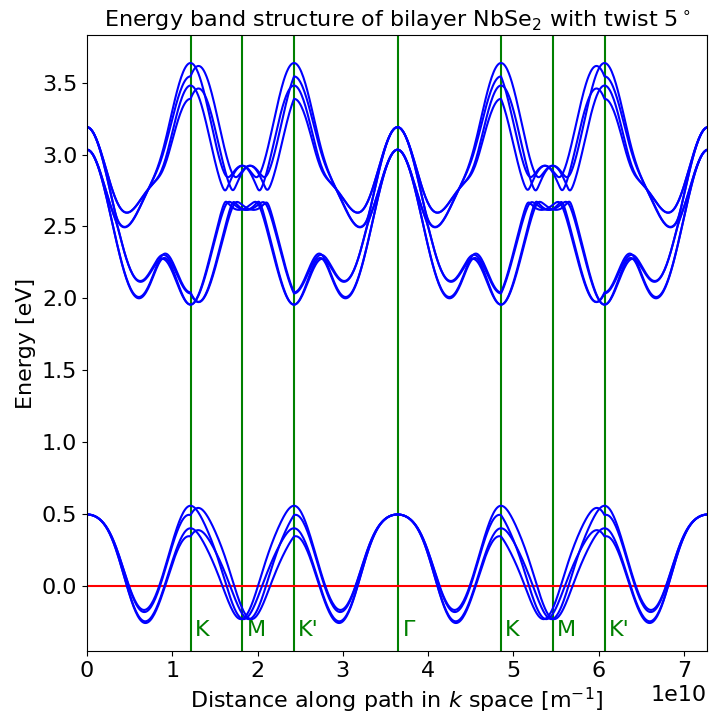
\includegraphics[width=0.95\textwidth]{bilayer_bands_5.png}
    \caption{
      Relative twist 5$^\circ$
    }
    \label{bilayer_bands_5}
  \end{subfigure}
  \hfill
  \begin{subfigure}[b]{0.475\textwidth}
    \centering
    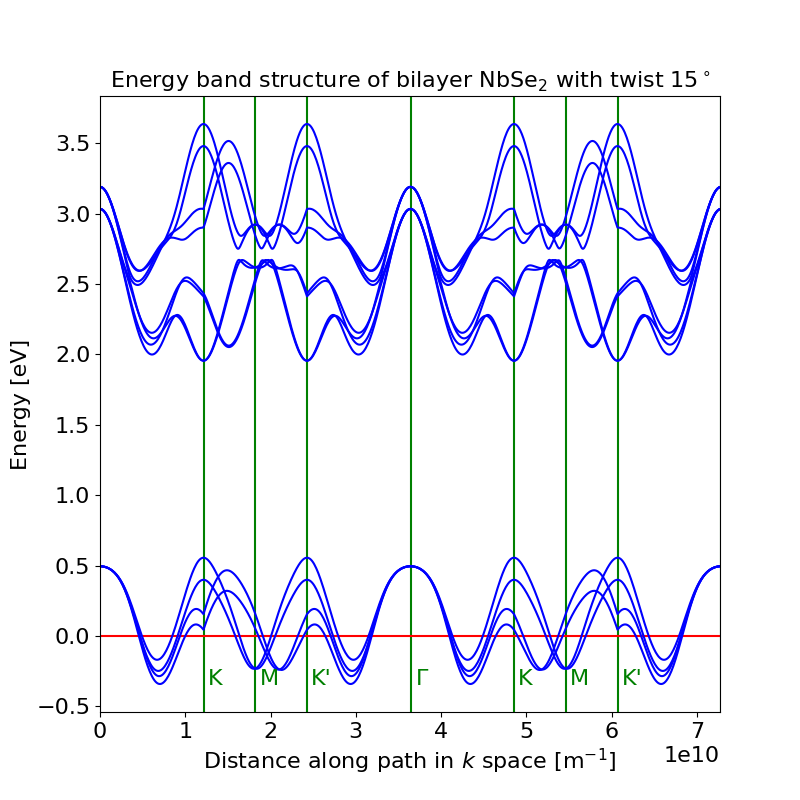
\includegraphics[width=0.95\textwidth]{bilayer_bands_15.png}
    \caption{
      Relative twist 15$^\circ$
    }
    \label{bilayer_bands_15}
  \end{subfigure}
  \vskip
  \baselineskip
  \begin{subfigure}[t]{0.475\textwidth}
    \centering
    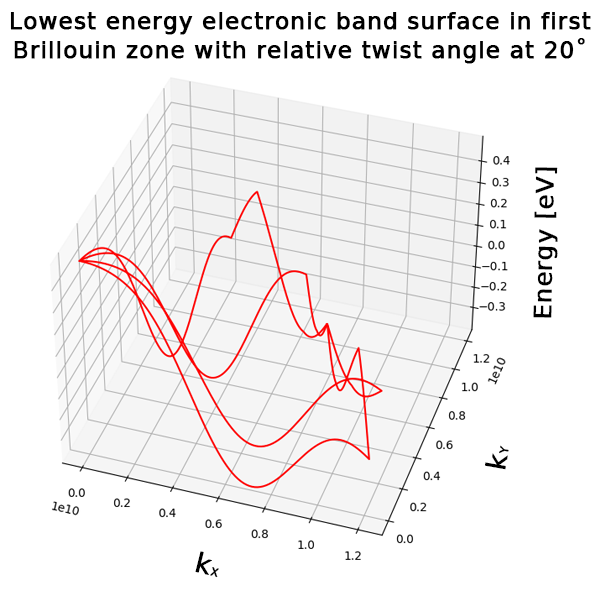
\includegraphics[width=0.95\textwidth]{surface_bands.png}
    \caption{
    }
    \label{surface_bands}
  \end{subfigure}
  \hfill
  \begin{subfigure}[t]{0.475\textwidth}
    \centering
    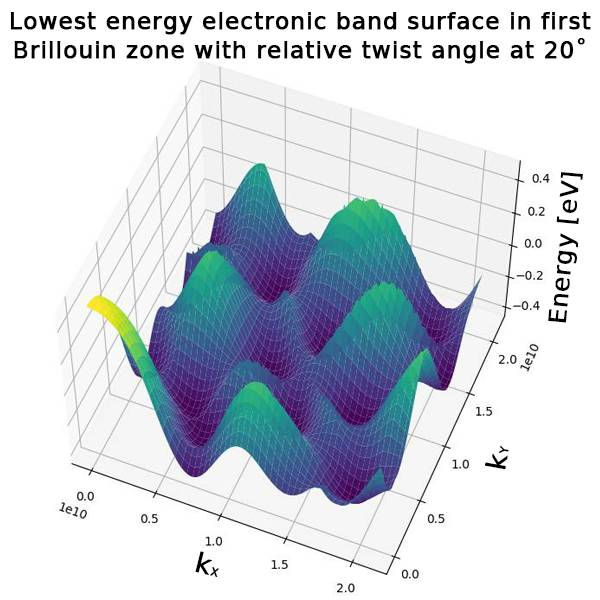
\includegraphics[width=0.95\textwidth]{surface.png}
    \caption{
    }
    \label{surface_plot}
  \end{subfigure}
  \caption{
    Bilayer band structure accounting for rotation at $5^\circ$ and $15^\circ$ — a) and b) respectively — with no inter-layer coupling. These graphs are equivalent to FIG \ref{monolayer_bands} for two monolayers at once, one with a relative twist to the other. The bands are sampled from two triangular paths in $k$ space, one after the other as in FIG \ref{heterostructure_BZ_path}. These paths join the critical points of symmetry in the Brillouin zone of the unrotated and then rotated lattices. A surface plot of the lowest energy band and that band sampled on the triangular path at twist $20^\circ$ are also shown in c) and d) respectively.
  }
  \label{bilayer_bands}
\end{figure*}

Following the monolayer bands, we construct a Hamiltonian of two layers, with one rotated at some twist angle $\theta$ as in (\ref{simple_bilayer_hamiltonian}). The graphs in FIG \ref{bilayer_bands} a) and b) show the electronic bands of both layers with $5^\circ$ and $15^\circ$ relative rotation respectively. The bands are sampled from the constructed path $\Gamma \rightarrow \Gamma \rightarrow \Gamma$ in $k$ space seen in FIG \ref{heterostructure_BZ_path}. The graphs in FIG \ref{bilayer_bands} a) and b) show 12 electronic bands, with 6 existing on each layer. Because of the construction of the paths in $k$ space taken, these graphs appear mirrored about the $\Gamma$ that separates the first and second triangular paths: there are always 6 bands which appear exactly as in FIG \ref{monolayer_bands}; the remaining 6 bands are those sampled from one of the triangular paths that is rotated relative to the layer they exist on. This results in discontinuities in the bands as the corners of the triangular paths are discontinuous in the 2D $k$ space plane.

The geometric reasoning for the apparent discontinuities is better seen in FIG \ref{bilayer_bands} c) and d), where at 20$^\circ$ rotation, the lowest energy band is shown on the triangular path it takes in c). The surface of the full 2D band in the same sampling region of the Brillouin zone is plotted in d). Again, nothing physically novel can be inferred from these graphs other than that the model up to this point is functional. They simply represent two sets of electronic states corresponding to two layers of NbSe$_2$, with no notion of interaction, coupling, or distance between layers - only a twist relative to each other. 

\subsection*{Interlayer tunneling}
With the model capable of describing a bilayer with relative twist, we now seek to introduce some interlayer interaction in the form of coupling by electron tunneling. From the relationship in (\ref{inter-layer_k_plus_G_M}) we found that for each state at point $k$ on one layer, there are a set of $k'$ on the other layer between which tunneling is allowed. We further reduced this set of $k'$ points to 7 points for practical computation by approximating the tunneling potential as a step function in (\ref{tunneling_potential}). To model the tunneling between these points, we expand the Hamiltonian to describe 84 states - using a fixed tunneling coefficient of 0.1 eV for the allowed interactions. The result is 84 eigenstates evaluated at each $k$, generating 84 electronic bands. In FIG \ref{bilayer_bands_coupled} we show the bands with energies near the Fermi level only. The perturbations introduced by the tunneling cause points where bands previously crossed (degeneracies) to separate into higher and lower energies as described in (\ref{perturbation_matrix}) and (\ref{perturbation_energy})
%
\begin{figure*}[t!]
\centering
  \begin{subfigure}[t]{0.475\textwidth}
    \centering
    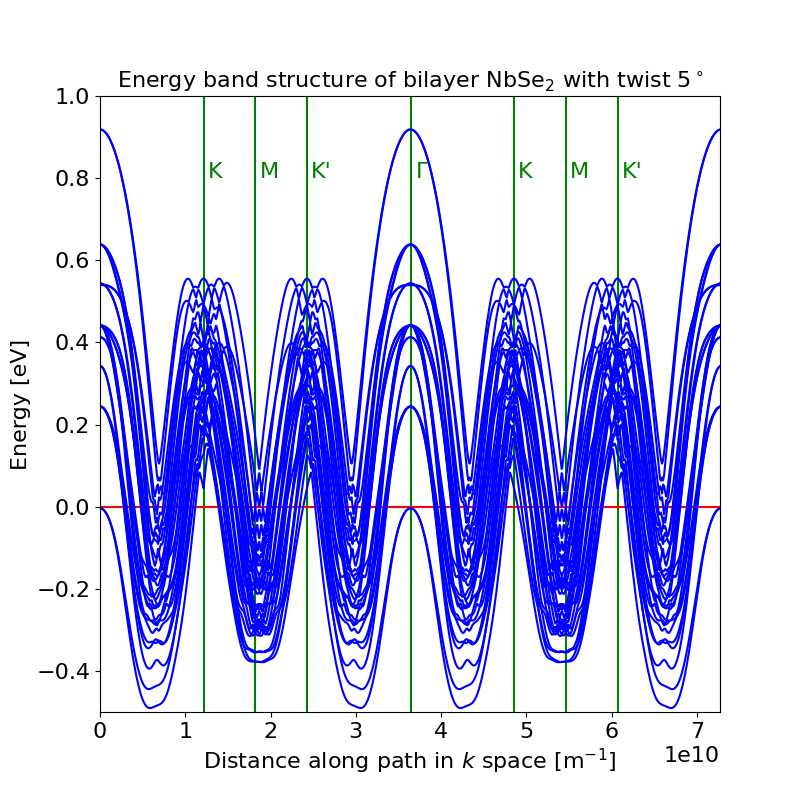
\includegraphics[width=0.95\textwidth]{bilayer_bands_5_coupled.png}
    \caption{
    }
    \label{bilayer_bands_5_coupled}
  \end{subfigure}
  \hfill
  \begin{subfigure}[t]{0.475\textwidth}
    \centering
    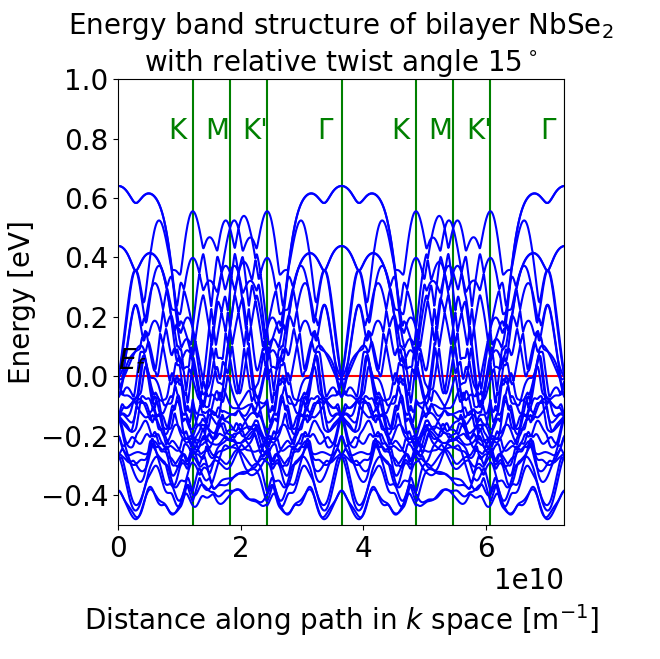
\includegraphics[width=0.95\textwidth]{bilayer_bands_15_coupled.png}
    \caption{
    }
    \label{bilayer_bands_15_coupled}
  \end{subfigure}
  \caption{Electronic bands near the Fermi level $E_f$ (shown in red) with interlayer coupling potential $t(k+G)$ set to 0.1 eV as in (\ref{tunneling_potential}). A basis of 84 electronic states is used to model the interlayer tunneling between allowed points, resulting in 84 electronic bands.
  }
  \label{bilayer_bands_coupled}
\end{figure*}

To better observe and understand the effects of interlayer tunneling we take a projection (inner product) of each of the 84 bands seen in FIG \ref{bilayer_bands_coupled} onto the lowest energy unperturbed states at $k_0 = k$ only (equivalent to those shown in FIG \ref{bilayer_bands}). We then examine the effects of varying the fixed coupling potential and interlayer twist angle in FIG \ref{bilayer_bands_projected_coupling} and FIG \ref{bilayer_bands_projected_rotation} respectively. In these graphs the opacity of the states (shown in red) is given by the numerical value of the projection
%
\begin{equation}
  \langle \psi_{i, k}'|\psi_{j, k} \rangle,
\end{equation}
%
where $\langle \psi_{i, k}'|$ is an eigenvector of the perturbed Hamiltonian at wavevector $k$ with index $i$ out of 84 states. $|\psi_{j, k} \rangle$ is an eigenvector of the unperturbed Hamiltonian (where $t(k+G)=0$) at wavevector $k$ with index $j$ out of the 12 eigenstates at $k_0$. This projection takes values between 0 and 1 and can be interpreted as the electron density in the perturbed state that still exists in the unperturbed state. In our graphs (FIG \ref{bilayer_bands_projected_coupling} and FIG \ref{bilayer_bands_projected_rotation}) and analysis we reduce the scope to eigenstates with energies near the Fermi level only.

Firstly we examine how altering the fixed coupling potential affects the band structure in FIG \ref{bilayer_bands_projected_coupling}, setting the nonzero value of our step function to $t(k+G) = 0.05, 0.1, 0.2 \text{ and } 0.4$ eV, if  $|G|\leq b$ and inter layer rotation to 15$^\circ$. There are two main observations: the interlayer coupling perturbation results in the splitting of the degenerate bands. This is best seen at the $\Gamma$ critical points where the two bands shown are almost indistinguishable in the unperturbed case. This degeneracy results in a large splitting of the bands seen in the projections, as predicted by the simpler two state model in (\ref{perturbation_matrix}) and (\ref{perturbation_energy}). As well as the low energy difference between the unperturbed states increasing the splitting of the bands, the strength of the coupling potential also increases the magnitude of the splitting.

The second observation is an increase in the perturbed electronic states that have a high projection (density) in the two low energy unperturbed states at $k_0$. This makes sense as the full band structures as in FIG \ref{bilayer_bands_coupled} contain hybrid states that exist partly as unperturbed states on the allowed $k'$ points. So as the tunneling potential is increased, we see a greater mixing of these perturbed hybrid states at other $k'$ with the two unperturbed states at $k_0$ shown.
%
\begin{figure*}[th]
\centering
  \begin{subfigure}[b]{0.475\textwidth}
    \centering
    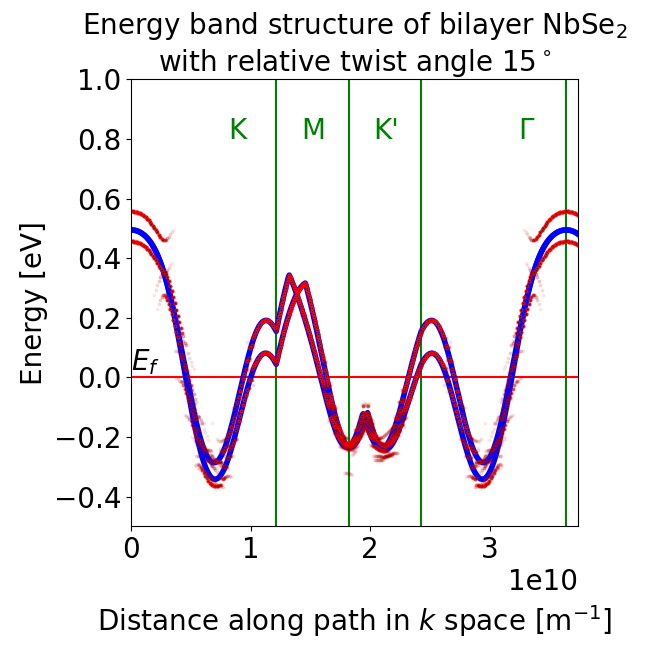
\includegraphics[width=0.95\textwidth]{0.05_coupling_15_deg.png}
    \caption{0.05 eV coupling}
    \label{bilayer_coupling_0.05}
  \end{subfigure}
  \hfill
  \begin{subfigure}[b]{0.475\textwidth}
    \centering
    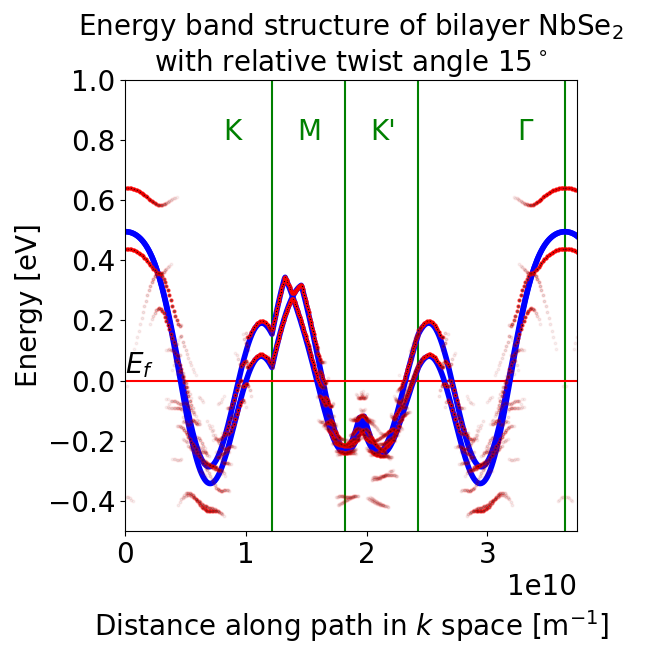
\includegraphics[width=0.95\textwidth]{0.1_coupling_15_deg.png}
    \caption{0.1 eV coupling}
    \label{bilayer_coupling_0.1}
  \end{subfigure}
  \vskip
  \baselineskip
  \begin{subfigure}[b]{0.475\textwidth}
    \centering
    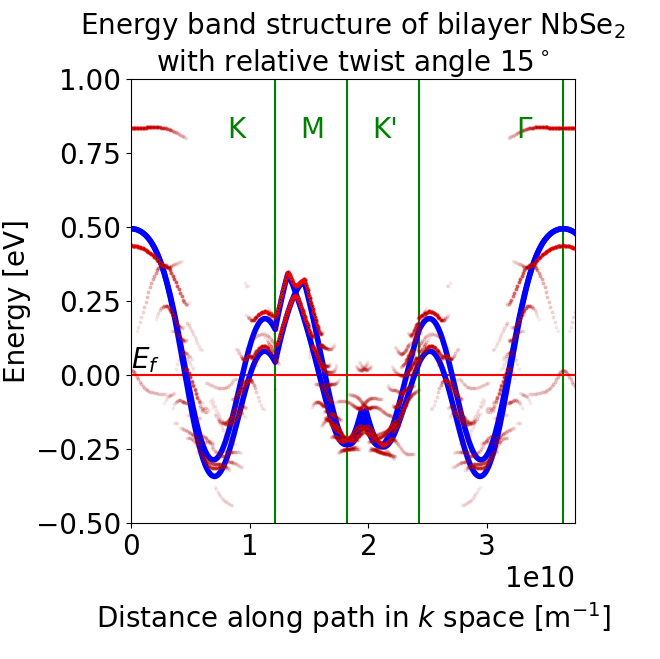
\includegraphics[width=0.95\textwidth]{0.2_coupling_15_deg.png}
    \caption{0.2 eV coupling}
    \label{bilayer_coupling_0.2}
  \end{subfigure}
  \hfill
  \begin{subfigure}[b]{0.475\textwidth}
    \centering
    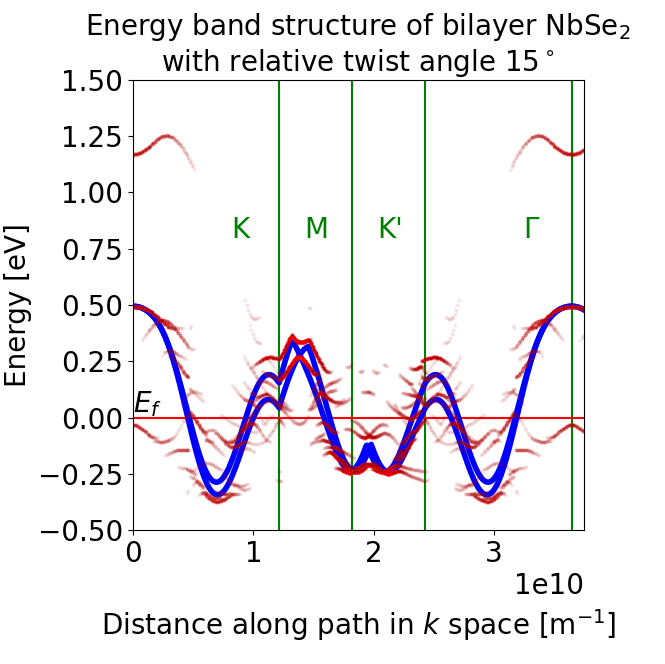
\includegraphics[width=0.95\textwidth]{0.4_coupling_15_deg.png}
    \caption{0.4 eV coupling}
    \label{bilayer_coupling_0.4}
  \end{subfigure}
  \caption{
    Altering the fixed interlayer coupling potential in (\ref{tunneling_potential}) at a twist angle of $15^\circ$. In experimentation we would expect to see coupling potentials approximately of order 0.1 eV \cite{Conte2019}. The perturbation introduced by the coupling causes the electronic bands to separate near degenerate points as in (\ref{perturbation_matrix}), (\ref{perturbation_energy}) and FIG \ref{splitting_bands}.
  }
  \label{bilayer_bands_projected_coupling}
\end{figure*}

We also examine the effects of altering the relative interlayer twist angle on the electronic band structure of the bilayer. In FIG \ref{bilayer_bands_projected_rotation} a selection of twist angles are shown with fixed 0.1 eV coupling potential. This coupling potential was chosen as it is consistent with other TMDC heterostructure coupling potentials \cite{Conte2019}. The twist angle has a significant effect on the electronic band structure, as seen in its projection onto the unperturbed states. At low twist angles we can observe the high degeneracy at $\Gamma$ causing the bands to split their energies by a few hundred meV. This effect is reduced at larger twist angles as fewer states are trying to occupy the same energies. Between the critical points we also see many states that have a non-zero projection onto the unperturbed states. This suggests that there is significant interlayer coupling at these points. Additionally at 5$^\circ$ and 20$^\circ$ we see that some bands near the Fermi level become flattened due to the perturbation effects. This can be better seen at a selection of twist angles in FIG \ref{flat_bands}. These flat bands arise at relatively large twist angles which is significant in the context of graphene, where the magic-angle is small at $1.1^\circ$ \cite{Cao2018, Bistritzer2011}. The significantly altered electronic band structure due to interlayer twist will have a drastic effect on the electronic properties of the bilayer, especially where flat bands are formed due to their high density of states.
%
\begin{figure*}[t]
\centering
  \begin{subfigure}[b]{0.475\textwidth}
    \centering
    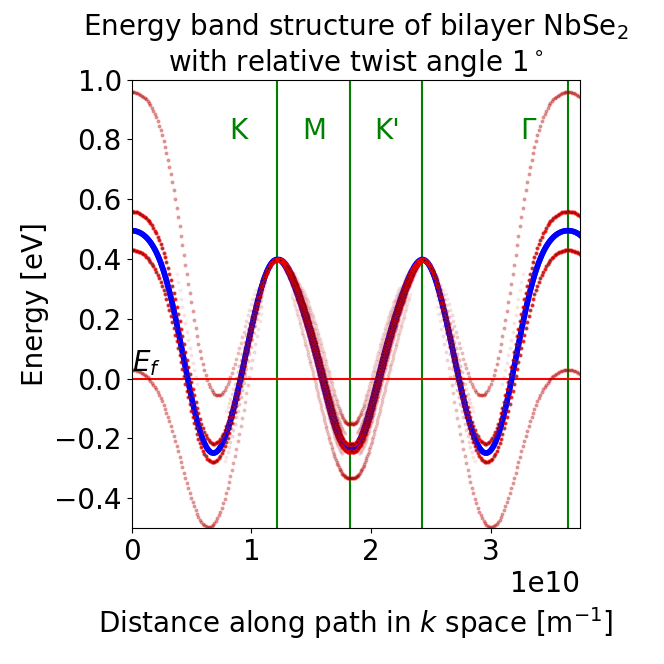
\includegraphics[width=0.95\textwidth]{1_deg_0.1_coupling.png}
    \caption{}
    \label{bilayer_rotation_1}
  \end{subfigure}
  \hfill
  \begin{subfigure}[b]{0.475\textwidth}
    \centering
    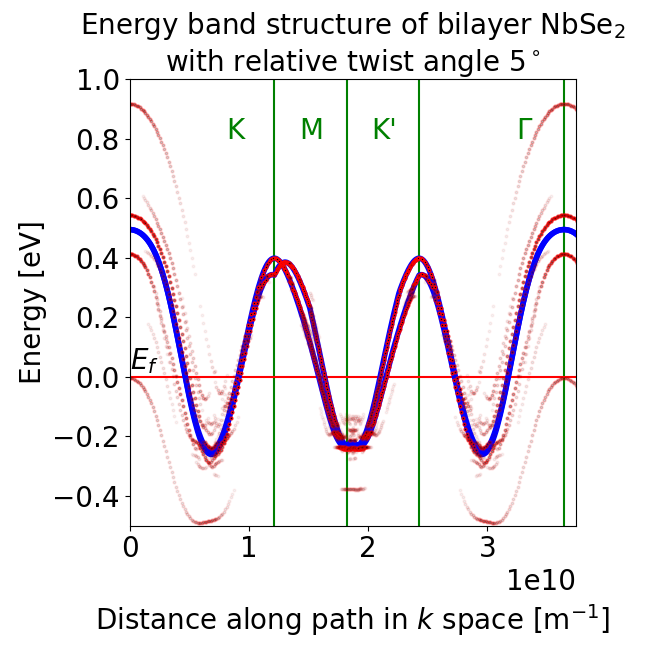
\includegraphics[width=0.95\textwidth]{5_deg_0.1_coupling.png}
    \caption{}
    \label{bilayer_rotation_5}
  \end{subfigure}
  \vskip
  \baselineskip
  \begin{subfigure}[b]{0.475\textwidth}
    \centering
    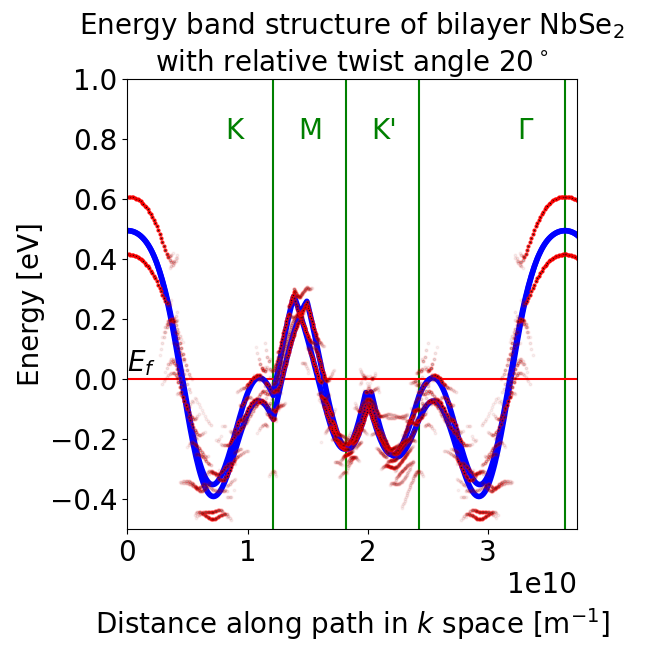
\includegraphics[width=0.95\textwidth]{20_deg_0.1_coupling.png}
    \caption{}
    \label{bilayer_rotation_20}
  \end{subfigure}
  \hfill
  \begin{subfigure}[b]{0.475\textwidth}
    \centering
    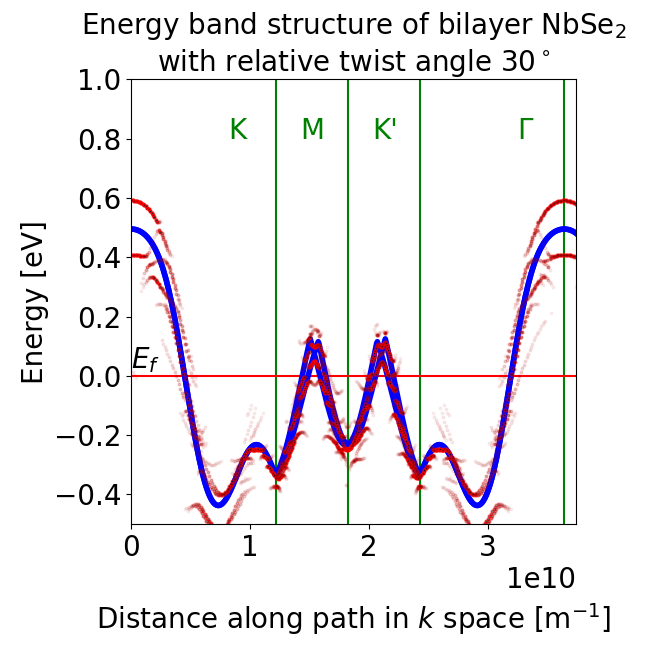
\includegraphics[width=0.95\textwidth]{30_deg_0.1_coupling.png}
    \caption{}
    \label{bilayer_rotation_30}
  \end{subfigure}
  \caption{
    Altering the relative interlayer twist angle at a fixed coupling potential of 0.1 eV. Some twist angles produce flat or nearly flat electronic bands associated with a high density of states.
  }
  \label{bilayer_bands_projected_rotation}
\end{figure*}
%
\begin{figure*}[t]
\centering
  \begin{subfigure}[b]{0.475\textwidth}
    \centering
    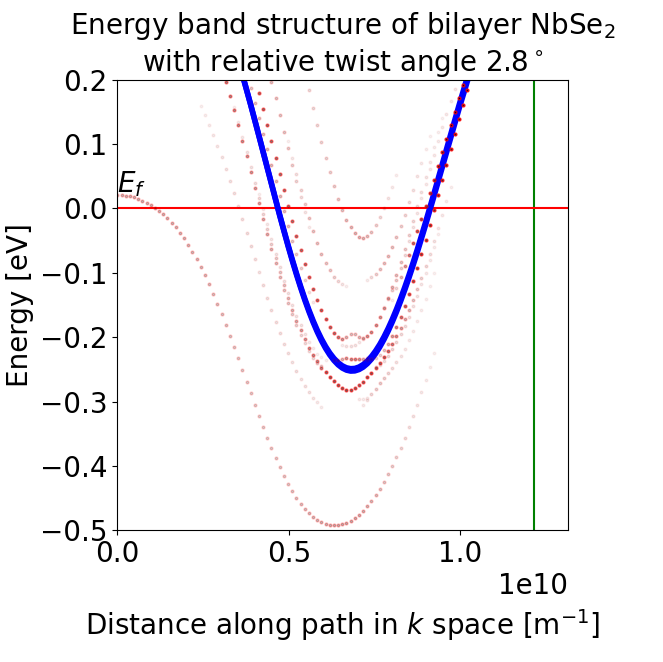
\includegraphics[width=0.95\textwidth]{flat_band_2.8.png}
    \caption{}
    \label{flat_band_2.8}
  \end{subfigure}
  \hfill
  \begin{subfigure}[b]{0.475\textwidth}
    \centering
    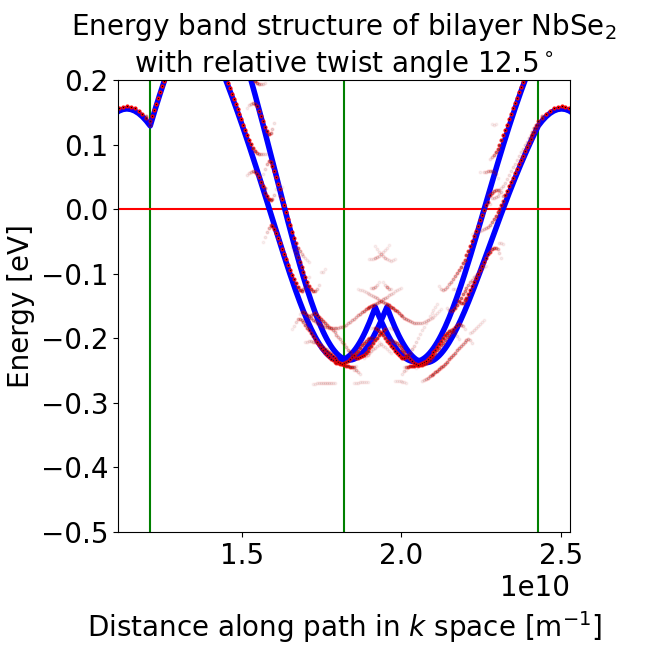
\includegraphics[width=0.95\textwidth]{flat_band_12.5.png}
    \caption{}
    \label{flat_band_12.5}
  \end{subfigure}
  \vskip
  \baselineskip
  \begin{subfigure}[b]{0.475\textwidth}
    \centering
    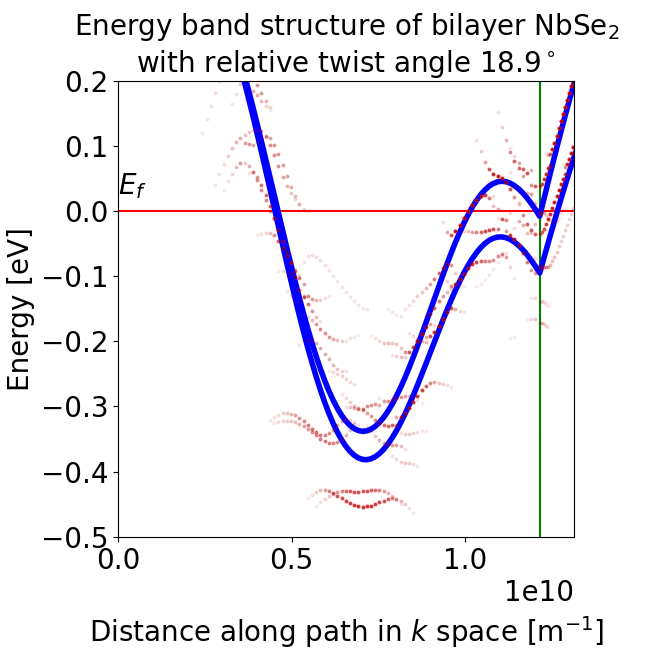
\includegraphics[width=0.95\textwidth]{flat_band_18.9.png}
    \caption{}
    \label{flat_band_18.9}
  \end{subfigure}
  \hfill
  \begin{subfigure}[b]{0.475\textwidth}
    \centering
    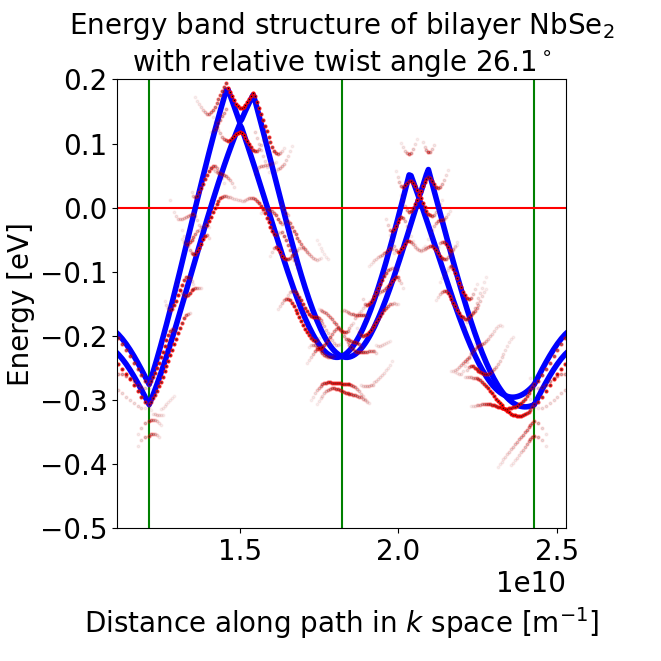
\includegraphics[width=0.95\textwidth]{flat_band_26.1.png}
    \caption{}
    \label{flat_band_26.1}
  \end{subfigure}
  \caption{Selected examples of almost flat electronic bands near the Fermi level}
  \label{flat_bands}
\end{figure*}

\section*{Discussion}
 The results we have presented offer a promising outlook on further research into twisted bilayer NbSe$_2$. In the greater context of TMDC heterostructures, they suggest that interlayer rotation can be treated as another degree of freedom in electronic devices that has a significant effect on their electronic properties \cite{Conte2019}. Improvements to the TBM and closer examination of the bands produced by twisted bilayers may present further interesting properties.

 The appearance of flat electronic bands near the Fermi level at some interlayer twist angles is significant. In graphene, flat bands are associated with superconductivity at the magic-angle of $1.1^\circ$ \cite{Cao2018, Bistritzer2011}. The tunability of electronic bands in van der Waals heterostructures could pave the way for new nanotechnological devices that exploit these tunable properties. Modern developments in twistronics could have wide ranging applications, from semiconductor technology and field effect transistors (FETs) to high temperature superconductors and quantum computing \cite{Ghuge2017, Geim2013, Gibney2019, Carr2017}. 

 We must acknowledge that significant approximations have been made in our TBM that raise doubt about the validity of the presented results. The most significant approximation is made in the interlayer coupling potential. In our numerical calculations we take a constant interlayer potential using the step function in (\ref{tunneling_potential}): where non-zero, the potential is of the order of magnitude predicted by density functional theory results in other TMDC heterostructures \cite{Conte2019}. This is far from physical as it doesn't take into account the interlayer distance or the relative distance between tunneling points. An alternate tunneling potential modelled by a Gaussian was suggested in (\ref{tunneling_potential_gaussian}), which would greatly improve the accuracy of the results presented, while keeping numerical computations simple. We propose fitting density functional theory results for tunneling potentials to this Gaussian. The tunneling potential model could also be improved upon by incorporating a description of the interlayer distance $z$, which we do not consider at all. Further improvements would go beyond a simple Gaussian to best describe the potential. Improving the tunneling potential model is likely to have a significant effect on the electronic bands and the results shown.

A more thorough description of interlayer tunneling potential would also aid in quantitatively justifying another approximation made in the allowed tunneling positions $k_{0, \cdots, 6}'$. We approximated (\ref{tunneling_potential_gaussian}) as (\ref{tunneling_potential}) by only allow tunneling to points of the first order $|G| \leq b$, assuming larger distances to have a smaller tunneling potential - yielding 7 allowed tunneling points. In our Hamiltonian at $k$, we consider the interlayer tunneling between $k$ and the 7 $k'$ points, these $k'$ points are also allowed to tunnel (between layers) to the $k$ points adjacent to them following the same criteria. The set of allowed $k'$ points could be expanded to a second ring, where $|G| \leq 2b$ using the Gaussian model. This would also allow further modelling of the tunneling between all of the $k'$ for a given $k$. Without a more quantitative (and physical) model of the tunneling potential, it is difficult to predict just how significant the effect on the overall band structure would be, which is itself a justification for further modelling.

Nonetheless, the results we have presented demonstrate that interlayer tunneling perturbations in twisted bilayers of NbSe$_2$ have a significant impact on the electronic properties of the material when compared to monolayer NbSe$_2$.

\section*{Conclusions}

We have demonstrated using a TBM that twisted bilayers of TMDC NbSe$_2$ have tunable electronic properties that differ significantly from its monolayer. Perturbation effects introduced by interlayer coupling result in the splitting of electronic bands at degenerate crossings. This splitting further goes on to create almost flat bands near the Fermi level. Flat bands are associated with a high density of states, which could induce superconductive or other non-trivial electronic states in the material. This work highlights the need for further research of TMDC heterostructures with interlayer twists, in particular those with NbSe$_2$ layers.

\section*{Acknowledgements}
I would like to acknowledge the contributions of my project partner Sanjana Reddy and my project supervisor Dr Marcin Mucha-Kruczynski. This work could not have been completed without their assistance, time, expertise and patience.

%%%References
\bibliographystyle{ieeetr}
%\bibliographystyle{bathx}
\bibliography{refs}

\clearpage

\section*{Appendix}

%\subsection*{Inter-layer tunneling Hamiltonian derivation}

\subsection*{Numerical implementation}
  Modelling, data analysis and plotting were performed in Python using the NumPy and Matplotlib libraries. All computations were performed on 64-bit processors either running Linux Mint 20.3 , Ubuntu Linux 20.04.4 LTS on WSL or Windows 10 home edition. Code and other details can be found on Github: "https://github.com/C-Birkett/Final-Year-Project".

\subsection*{Animation across twist angles}
Please visit the Github for an animation of the electronic bands at the Fermi level over twist angles from $0^\circ \text{ to } 30^\circ$.

  %\textbf{Note: }

  %Code example
\begin{lstlisting}

\end{lstlisting}

\end{document}
